\chapter{Reinforcement Learning}
\section{Introduction}
The robot controls its motors using the artificial neural networks and the deep deterministic policy gradient (DDPG) algorithm, produced by Lillicrap et al. The system runs in Python 3, leaning heavily on the TensorFlow library.

\section{Reinforcement Learning Background}
Reinforcement learning (RL) is a subset of machine learning that aims to solve control and action selection problems rather than to perform classification or data clustering. Most reinforcement learning problems involve six main elements: an actor, the environment, rewards, a policy, a value function, and sometimes a model. An actor (sometimes called an agent) takes actions in an environment which returns a state and reward, illustrated in Figure \ref{fig:actor_env_loop}. The actor's primary goal is to maximize the accumulated reward received from the environment. A policy determines which actions the actor takes given the current state and can be considered a mapping from state to action. The value function indicates the long-term reward expected from a state so even if a state only has a small immediate reward, it may possess high value since it leads to high reward states. Some algorithms involve a model of the environment, allowing prediction of the next state from the current state and action. Table \ref{tab:rl_defs} summarizes some common terms and definitions used in the reinforcement learning literature.
\begin{figure}[H]   % [h] means here
	\centering 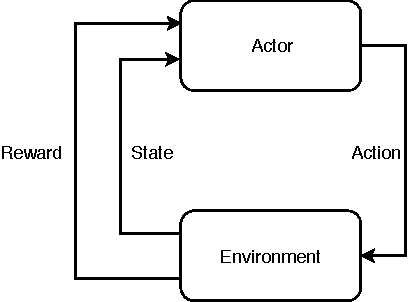
\includegraphics[width=3in, height=3.85in, keepaspectratio]{figures/actor_env_loop.pdf}
	\caption{Actor-Environment Feedback Loop}\label{fig:actor_env_loop}
\end{figure}
Actors strive to maximize the long-term discounted reward, $G_t$, where the subscript $t$ denotes the time step. In RL problems with a definitive end (denoted by $t=T$) such as a game of chess, $G_t$ is finite and can be calculated simply as the sum of all future rewards (\ref{eq:Gt_simple}). 
\begin{equation}
	\label{eq:Gt_simple}
	G_t=R_{t+1}+R_{t+2}+\dots + R_{T}=\sum_{k=t}^{T-1} R_{k+1}
\end{equation}
However, continuous problems such as maintaining the temperature of a refrigerator have no maximum time step and therefore, a possibly infinite $G_t$. The introduction of a discount factor, $\gamma$, makes such a situation manageable. The discount factor weights the worth of future rewards exponentially by their distance into the future. It ranges from 0 to 1 where 0 completely devalues future rewards while a discount factor of 1 weights all future rewards equally. In practice, the discount factor is less than 1 in order to allow $G_t$ to converge \cite{sutton_2017}. The discount factor can be considered a knob setting the algorithm between myopic (short-sighted, only values immediate rewards) and far-sighted (willing to sacrifice immediate reward for greater long-term return).
\begin{equation}
	G_t=R_{t+1}+\gamma R_{t+2}+\gamma^2 R_{t+3} + \dots = \sum_{k=0}^{\infty} \gamma^k R_{t+k+1}
\end{equation}
The value function is the expected long-term reward as function of the state under a certain policy $\pi$ (\ref{eq:value_func}). The $\mathbb{E}_\pi$ operator evaluates the expected value provided the actor follows policy $\pi$.
\begin{equation}
	\label{eq:value_func}
	V_\pi(s)=\mathbb{E}_\pi [G_t | S_t =s]
\end{equation}
Core to many RL algorithms, the Q-function or action-value function is the expected long-term reward as a function of the state \textbf{and action} under a certain policy $\pi$ (\ref{eq:q_func}). The important distinction from the value function is dependency on the action. 
\begin{equation}
	\label{eq:q_func}
	Q_\pi(s,a)=\mathbb{E}_\pi [G_t | S_t =s, A_t=a]
\end{equation}

\LTXtable{\textwidth}{tables/tab_rl_defs.tex}

\section{Reinforcement Learning Algorithms}
Many reinforcement learning algorithms have been applied to control including Q-Learning, State-Action-Reward-State-Action (SARSA), and Deep Deterministic Policy Gradient (DDPG), among others. Note that these methods differ from evolutionary algorithms in that they actively learn as they interact with the environment.

RL algorithms can be classified by their use of models (model-based vs. model-free) and actor policy (on-policy vs. off-policy). Model-based strategies first develop a model of the environment and then use a planning algorithm with the model to create a controller. Model-free algorithms forgo the model entirely and find good policies directly. 

On-policy algorithms learn the policy followed by the actor while off-policy strategies learn a policy different from the one followed by the actor. Various policies exist but the most commonly referred to in the literature include optimal, greedy, $\epsilon$-greedy, and random. The optimal policy $\pi_*$, by definition, produces greater value for every possible state than any other policy $\pi$, expressed in (\ref{eq:optimalpol}) where $\mathcal{S}$ is the set of all possible states. An actor using the greedy policy always takes the action with the highest value or Q-value depending on implementation. The $\epsilon$-greedy policy tells an actor to pick the greedy action with probability $1-\epsilon$ and a random action with probability $\epsilon$. Finally, an actor under the random policy always takes random actions.
\begin{equation}
	\label{eq:optimalpol}
v_{\pi_*}(s) \geq v_{\pi}(s), \forall s \in \mathcal{S}
\end{equation}

\subsection{Q-Learning}
Q-Learning is an off-model, off-policy algorithm that estimates the Q-function of the environment. The Q-function represents the "quality" of every possible action in every possible state. For example, imagine a game of tic-tac-toe as shown in Figure \ref{fig:tictactoe}. Each of the nine spaces can take one of three values (blank, X, or O) so the game has $3^9=19,683$ possible states (although some states are not achievable as the game would end once a player gets three in a row). Given a particular state, the Q-function returns the quality of each possible action the player could take. Therefore, the optimal action to take is simply the one with the highest Q-value. 
\begin{figure}[H]   % [h] means here
	\centering 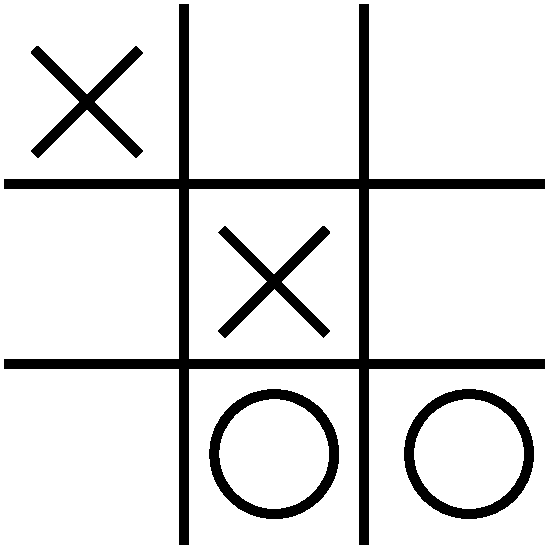
\includegraphics[width=3in, height=3.85in, keepaspectratio]{figures/tictactoe.pdf}
	\caption{A Game of Tic Tac Toe}\label{fig:tictactoe}
\end{figure}
Clearly, the Q-function always exists but not necessarily in an analytic or obvious form. So-called tabular Q-learning methods use a 2-D matrix to represent the Q-function with rows for all possible states and columns for all possible actions. The table is initialized with guesses (or all elements set to 0) and iteratively updated to approximate the true Q-function using the Bellman equation (\ref{eq:bellman}).
\begin{equation}
	\label{eq:bellman}
	Q(s,a)=R(s) + \gamma (\text{max}_{a'}(Q(s',a')))
\end{equation}
To improve convergence, Equation \ref{eq:bellman} is modified to include the learning rate $\alpha$. The pseudocode for Q-learning presented by Sutton is reproduced below. The $\text{max}_{a'}()$ operator maximizes its argument with respect to $a'$.
\begin{center} \begin{tabular}{|p{0.9\linewidth}|}\hline % or any other width
Initialize $Q(s,a)$ arbitrarily. \\
Repeat (for each episode): \\
\qquad Initialize $s$\\
\qquad Repeat (for each step of episode):\\
\qquad \qquad Choose $a$ from $s$ using policy derived from $Q$ (e.g., $\epsilon$-greedy)\\
\qquad \qquad Take action $a$, observe $r$, $s'$\\
\qquad \qquad $Q(s,a)\gets (1-\alpha)Q(s,a) + \alpha [r + \gamma \text{max}_{a'}Q(s',a')]$\\
\qquad \qquad $s \gets s';$\\
\qquad until $s$ is terminal \\
\hline
\end{tabular} \end{center}
Notice the algorithm updates the Q-value, $Q(s,a)$, from the Q-value of the next state and greedy policy action, $\text{max}_{a'}Q(s',a')$, regardless of the policy and action taken by the actor. This characteristic makes Q-learning an off-policy algorithm. The Q-value for a particular state and action only updates when the actor visits said state and action so the actor must still explore (not always take greedy actions) for Q-learning to converge.

Clearly, the tabular Q method quickly becomes unfeasible for more complex problems, especially when the states or actions become continuous rather than discrete. When the action or state spaces are continuous, the algorithm must discretize them, forcing a tradeoff between resolution and tractability. For the tic-tac-toe example, the table would be 19,683 rows by 9 columns for a total of 177,147 Q-values while the Q-value table for a game of chess would possess more elements than there are atoms in the known universe.

\subsection{State-Action-Reward-State-Action (SARSA)}
SARSA is an on-policy algorithm similar which shares many characteristics with Q-Learning. The name comes from the fact that the Q update equation uses the current state and action as well as the next reward, state, and action. The pseudocode for SARSA presented by Sutton is reproduced below:
\begin{center} \begin{tabular}{|p{0.9\linewidth}|}\hline % or any other width
Initialize $Q(s,a)$ arbitrarily. \\
Repeat (for each episode): \\
\qquad Initialize $s$\\
\qquad Choose $a$ from $s$ using policy derived from $Q$ (e.g., $\epsilon$-greedy)\\
\qquad Repeat (for each step of episode):\\
\qquad \qquad Take action $a$, observe $r$, $s'$\\
\qquad \qquad Choose $a'$ from $s'$ using policy derived from $Q$ (e.g., $\epsilon$-greedy)\\
\qquad \qquad $	Q(s,a)\gets (1-\alpha)Q(s,a) + \alpha [r + \gamma Q(s',a')]$\\
\qquad \qquad $s \gets s'; a \gets a'$;\\
\qquad until $s$ is terminal \\
\hline
\end{tabular} \end{center}
Unlike Q-learning, SARSA updates Q-values from the next state and next action $Q(s',a')$, making it an on-policy strategy. Like Q-learning the actor must take exploratory actions for the algorithm to converge.

\subsection{Deep Q Network (DQN)}
Deep Q Networks aim to solve the problem with Q-learning in two ways: the inability to handle situations with large state and action spaces and the inability to generalize learnings to new situations. As mentioned previously, maintaining Q-values for the entire state and action space of a complex problem requires enormous memory. The second problem has to do with how the Q-value table updates. In both Q-learning and SARSA, the algorithms iteratively update Q-values for visited (state, action) pairs. However, to fully update the Q-value table means exploring every possible state and action combination multiple times, a non-trivial task. In other words, the algorithms cannot provide reasonable Q-value estimates for unvisited situations.

To overcome these limitations, DQN replaces the tabular Q concept with an artificial neural network (ANN) where the inputs are the state and action and the output is the Q-value. The Q-network is denoted as $Q(s,a;\theta_i)$ where $\theta_i$ represents the network weights. The loss function (\ref{eq:dqn_loss_func}) is the squared error between the Q-network output and the "target Q-value" as defined by the Bellman equation, $y_j = r + \gamma \text{max}_{a'}Q(s', a';\theta^-_i)$  \cite{Mnih_2015}. For complete clarity, $Q(s,a;\theta^-_i)$ represents an identical but separate copy of Q-network $Q(s,a;\theta_i)$ except with weights $\theta^-_i$ from a previous iteration, explained later.
\begin{equation}
	\label{eq:dqn_loss_func}
L_i(\theta_i) = (r + \gamma \text{max}_{a'}Q(s', a';\theta^-_i)-Q(s,a;\theta_i))^2
\end{equation}
To assist DQN training, Mnih et. al. used a technique called experience replay. As the actor explores within environment, the algorithm records the state, action taken, reward, and next state at each time step into a so-called experience replay buffer. After collecting a minimum number of experiences, the artificial neural network trains from data sampled randomly from the buffer, hence the name "experience replay". The technique removes time correlations in the training data, improving convergence, and also allows experience reuse, advantageous when obtaining data is difficult or costly.

The second technique Mnih et. al. used to counter training instability involves generating target Q-values, $y_j$, from an identical but separate ANN, called the target Q-network $\hat{Q}$ with weights $\theta^-_i$. In effect, this creates a time delay between when the weights of $Q$ are updated and when those updates affect the policy and target Q-network, reducing the likelihood of policy instability. 

For example, using a 64 transition mini-batch, the network samples 64 transitions from the experience replay buffer and trains the network $Q$ with 64 iterations as in \ref{eq:dqn_loss_func}. After, the target network $\hat{Q}$ clones the weights $\theta_i$ from $Q$ and the process repeats.

DQN replaced the tabular Q with an artificial neural network to solve RL problems with large Q spaces. However, the policy still uses a discrete action space, posing an issue for situations requiring continuous actions. For example, a system with five actions discretized into only four bits each already produces 32,768 different actions. Policy gradient methods can overcome this limitation.

\subsection{Stochastic Policy Gradient Method}
Q-Learning, SARSA, and DQN are value-based methods as they rely on finding the environment's underlying Q-function and produce a policy to maximize Q. Policy gradient methods find the optimal policy directly which makes them policy-based strategies \cite{sutton_policygrad}. In fact, DeepMind's AlphaGo famously defeated grandmaster Go player Fan Hui in 2015 and Lee Sedol in 2016 using an algorithm incorporating a policy gradient method, definitively proving its viability \cite{silver_2017}.

The underlying premise of stochastic policy gradients is simple: get a state, take a particular action with probability $P(a)$, and record the reward. If the reward is "good", increase the probability of taking that action or decrease it if the reward is "bad". Note that the terms "good" and "bad" are intentionally vague as to not constrain them to one particular interpretation. After many iterations, the actor will most likely take actions that produce good rewards. But of course, not all is so simple. Much like the so-called "butterfly effect" \cite{Lorenz_1963}, a single action can cascade into a multitude of unknown futures meaning the worth of a particular action cannot be determined by the immediate reward produced. 

Instead, the rewards are accumulated for a long period in episodes, at the end of which actions are judged based on the total reward. Now, a different issue arises: the credit assignment problem \cite{fu_2008}. If an episode contains 1,000 actions, which ones ultimately produced the good reward and which were inconsequential or detrimental? Rather than determining the individual actions responsible, the algorithm deems all actions in an episode culpable so if the episode outcome is good, all actions taken become more likely and if not, the inverse occurs \cite{karpathy_2016}. Like AlphaGo, many policy gradient implementations use an artificial neural network where the inputs are states and outputs are action probabilities \cite{silver_2017}. Therefore, the act of making actions more or less probable is carried out with the standard back-propagation algorithm where the gradient is adjusted by normalized episodic reward \cite{karpathy_2016}.
%A more concrete implementation is shown below in pseudocode where $P(s,a,\theta)$ represents the parametrized probability of action $a$ in state $s$ for all possible states and actions, $\theta$ represents the parameters controlling the probability distribution:
%\begin{center} \begin{tabular}{|p{0.9\linewidth}|}\hline % or any other width
%Initialize $P(s,a,\theta)$ arbitrarily. \\
%Repeat until satisfactory performance: \\
%\quad Policy rollout n times (typ. 20 to 100): \\
%\quad \quad Initialize $s$\\
%\quad \quad Repeat (for each step of episode):\\
%\quad \quad \quad Stochastically choose $a$ from $s$ using policy derived from $P(s,a,\theta)$\\
%\quad \quad \quad Take action $a$, observe $s'$, accumulate $r$\\
%\quad \quad \quad $s \gets s'$;\\
%\quad \quad until $s$ is terminal \\
%\quad Normalize the $r$ from n policy rollouts. \\
%\quad 
%\hline
%\end{tabular} \end{center}

\subsection{Deterministic Policy Gradient Method (DPG)}
The deterministic policy gradient method (DPG), developed by Silver et. al., shares the same foundation as stochastic policy gradients, but instead of representing the policy as a probability distribution, the policy deterministically chooses actions from the given states \cite{silver_lever_heess_degris_wierstra_riedmiller}. Silver et. al. have shown that the DPG is actually a limiting case of stochastic policy gradients where the policy distribution variance is 0. Another key difference is that while the stochastic policy gradient integrates over the state and action spaces, the DPG only integrates over the state space. Consequently, the stochastic case requires more samples to compute. Finally, the stochastic policy inherently chooses exploratory actions due to its probabilistic nature so Silver developed an off-policy learning algorithm using a stochastic policy to ensure sufficient exploration despite producing a deterministic policy.

\subsection{Deep Deterministic Policy Gradient (DDPG)}
The deep deterministic policy gradient algorithm, developed by Lillicrap et. al., is a model-free, off-policy actor-critic strategy based on the Silver et. al.'s DPG algorithm combined with learnings from Mnih et. al.'s work on the DQN algorithm \cite{silver_lever_heess_degris_wierstra_riedmiller}\cite{lillicrap_2016}\cite{Mnih_2015}. DDPG improves on DPG by representing the actor policy with an ANN and applying the experience replay and target network techniques from DQN. 

Additionally, Lillicrap et. al. adapted batch normalization from Ioffe's work to allow ANN hyper-parameter generalization for environments with features of varying magnitude \cite{2015arXiv150203167I}; each feature in a minibatch is normalized to unit mean and variance. In their implementation, batch normalization was applied to network inputs, all layers of the policy network, and all layers of the Q network before the action input (detailed later).

To ensure adequate exploration, Lillicrap et. al. added Ornstein-Uhlenbeck process noise to the policy output $\mu(s_t | \theta^\mu_t)$ to create the exploration policy $\mu'(s_t)$ as shown in Equation \ref{eq:exploration_policy} \cite{lillicrap_2016}. The Ornstein-Uhlenbeck process satisfies the condition shown in Equation \ref{eq:ornstein-uhlenbeck} where $x_t$ is the process position at time $t$, $\theta$ and $\sigma$ are parameters, and $W_t$ is the Weiner process \cite{uhlenbeck_ornstein}. The process produces random, time-correlated values that drift toward a long-term mean, in this case 0.
\begin{equation}
\label{eq:exploration_policy}
\mu'(s_t) = \mu(s_t | \theta^\mu_t) + \mathcal{N}
\end{equation}
\begin{equation}
\label{eq:ornstein-uhlenbeck}
dx_t = \theta(\mu-x_t) dt + \sigma dW_t, \theta>0, \sigma>0
\end{equation}

Lillicrap et. al. used DDPQ to solve over 20 different simulated physics environments such as cartpole swing-up and driving using the same network architecture and hyper-parameters, demonstrating the generalizability of the technique. Although the approach required about 2.5 million steps of experience to solve most problems, it needed 20 times less than DQN.

\section{DDPG Implementation}
All code is implemented in Python 3.6 and uses libraries from TensorFlow \cite{tensorflow} and OpenAI Gym \cite{openaigym}. An implementation of the DDPG algorithm from Patrick Emami's wonderful reinforcement learning primer formed the springboard from which 


\subsection{title}


\section{Training}

\section{Testing}

\section{Results}

\begin{figure}
	\begin{tabular}{ccc}
		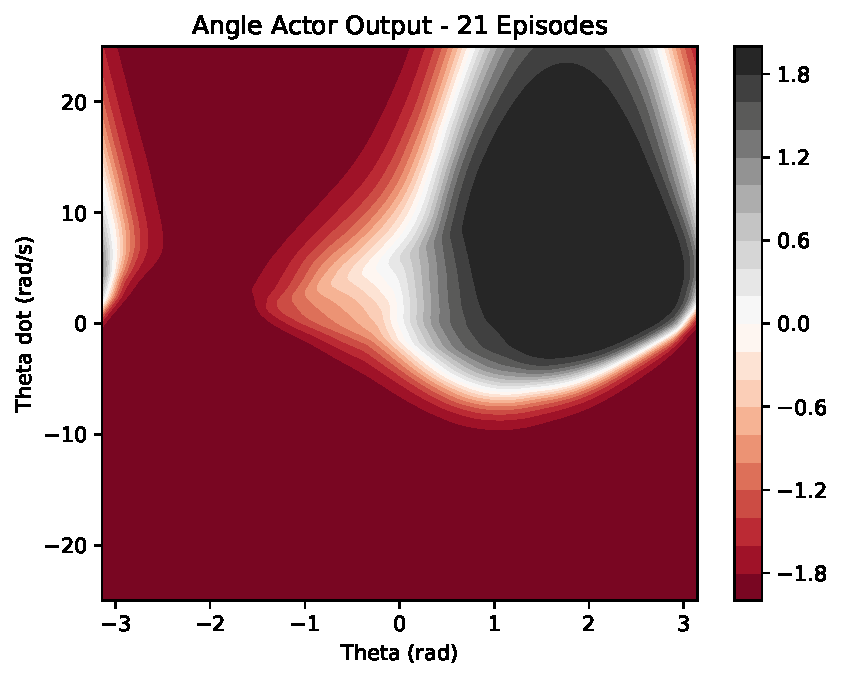
\includegraphics[width=65mm]{figures/train_figs/angle_actor/Actor0_21.pdf} &  
		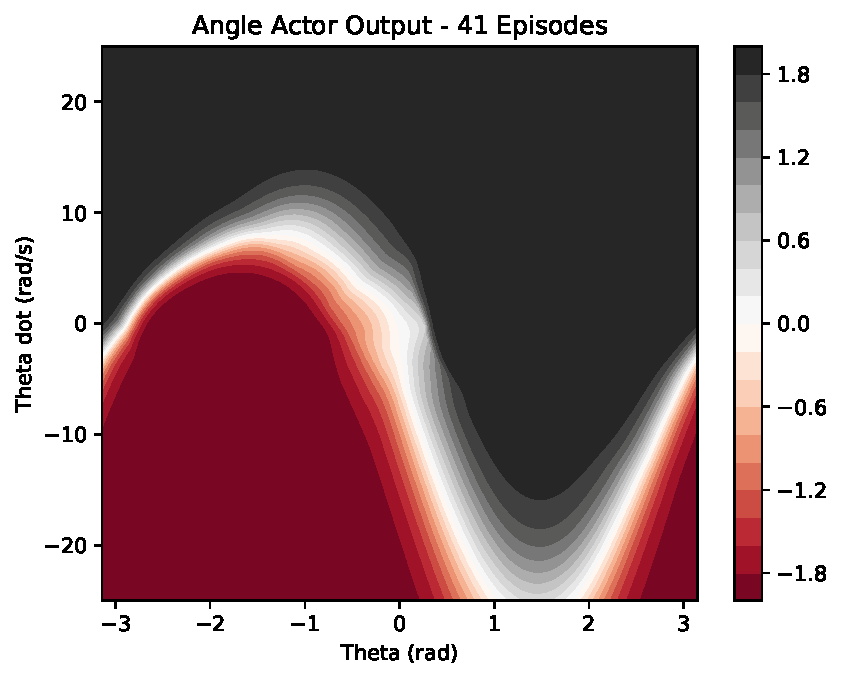
\includegraphics[width=65mm]{figures/train_figs/angle_actor/Actor0_41.pdf} \\
		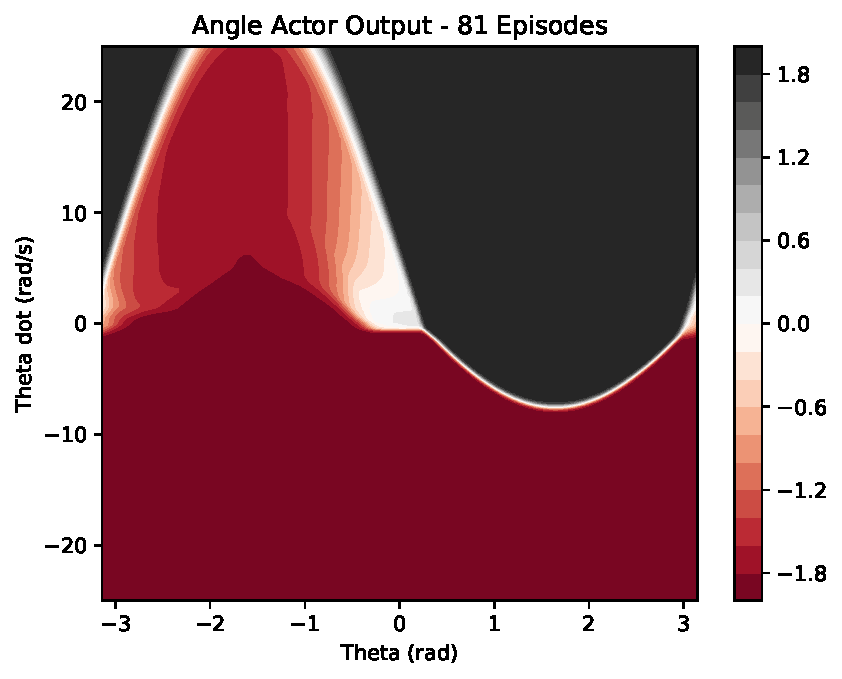
\includegraphics[width=65mm]{figures/train_figs/angle_actor/Actor0_81.pdf} &   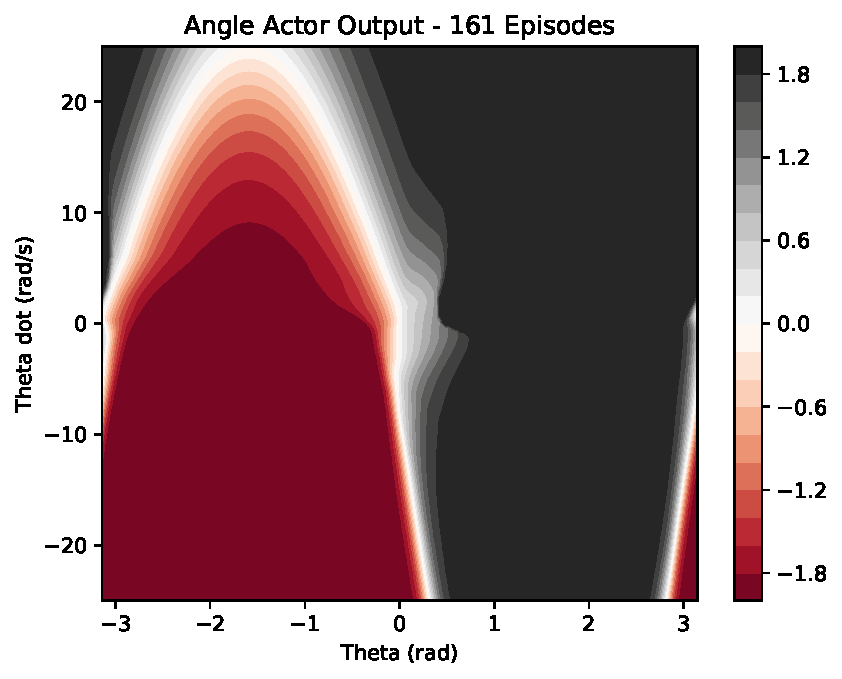
\includegraphics[width=65mm]{figures/train_figs/angle_actor/Actor0_161.pdf} \\
		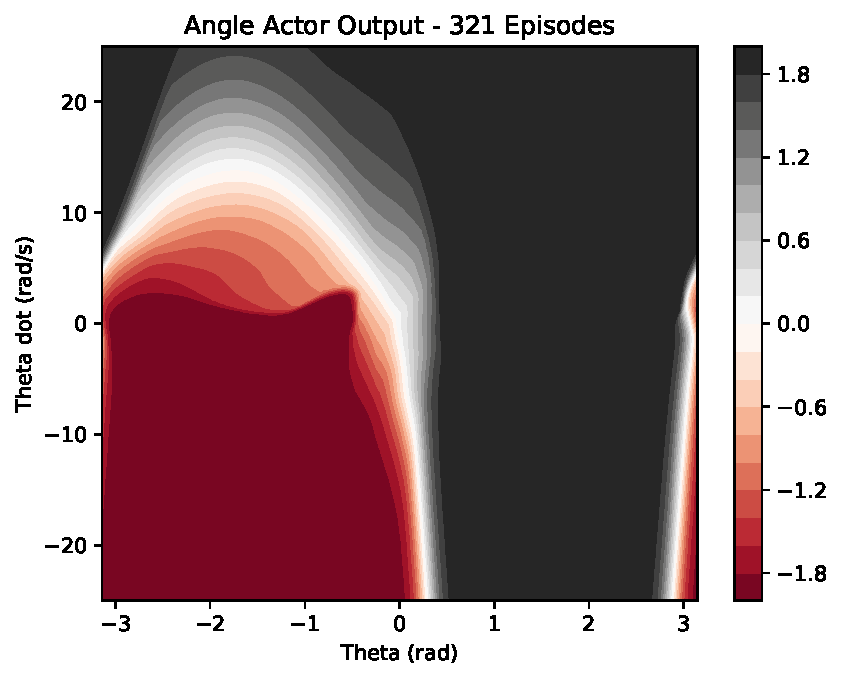
\includegraphics[width=65mm]{figures/train_figs/angle_actor/Actor0_321.pdf} &   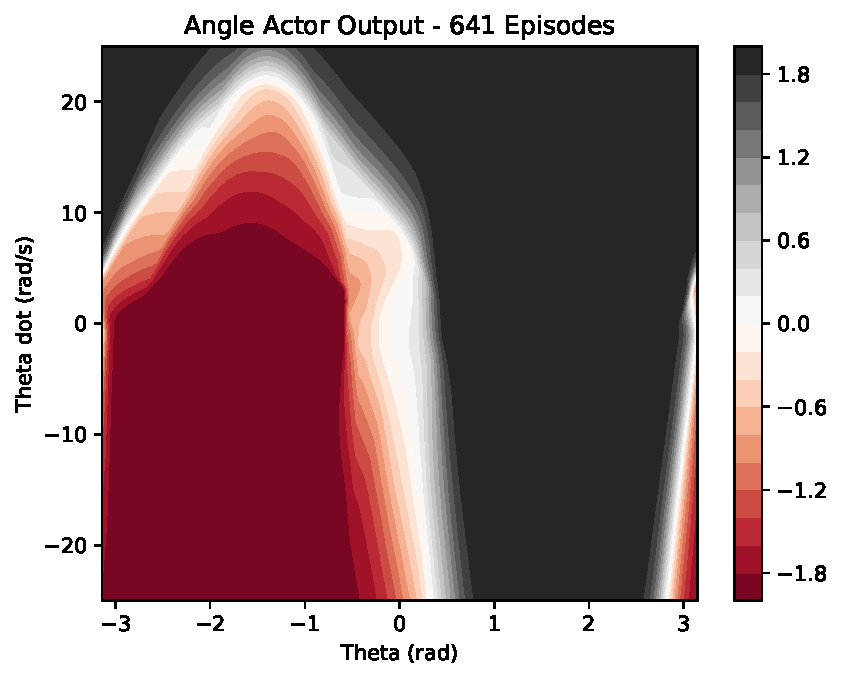
\includegraphics[width=65mm]{figures/train_figs/angle_actor/Actor0_641.pdf} \\
		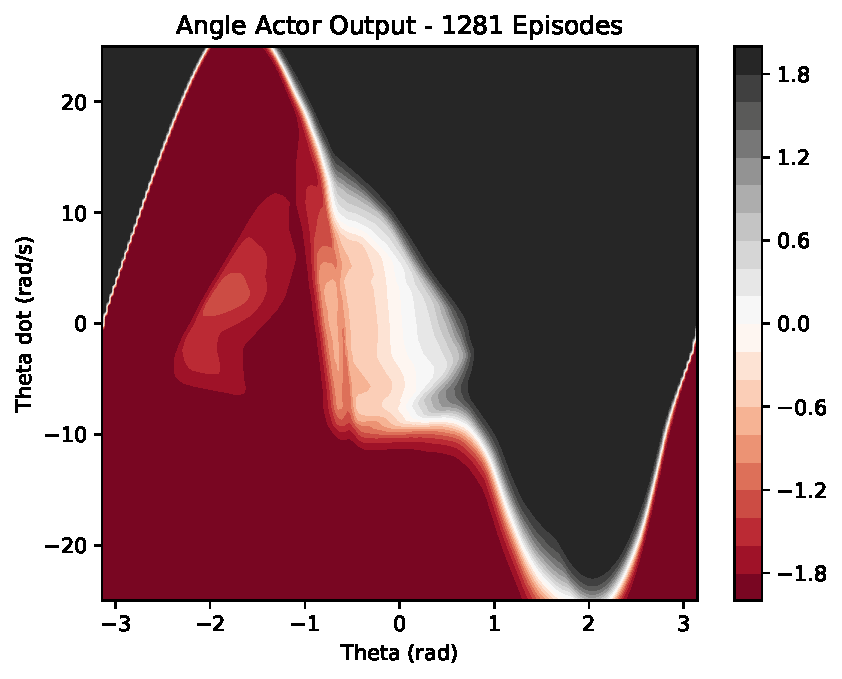
\includegraphics[width=65mm]{figures/train_figs/angle_actor/Actor0_1281.pdf} &   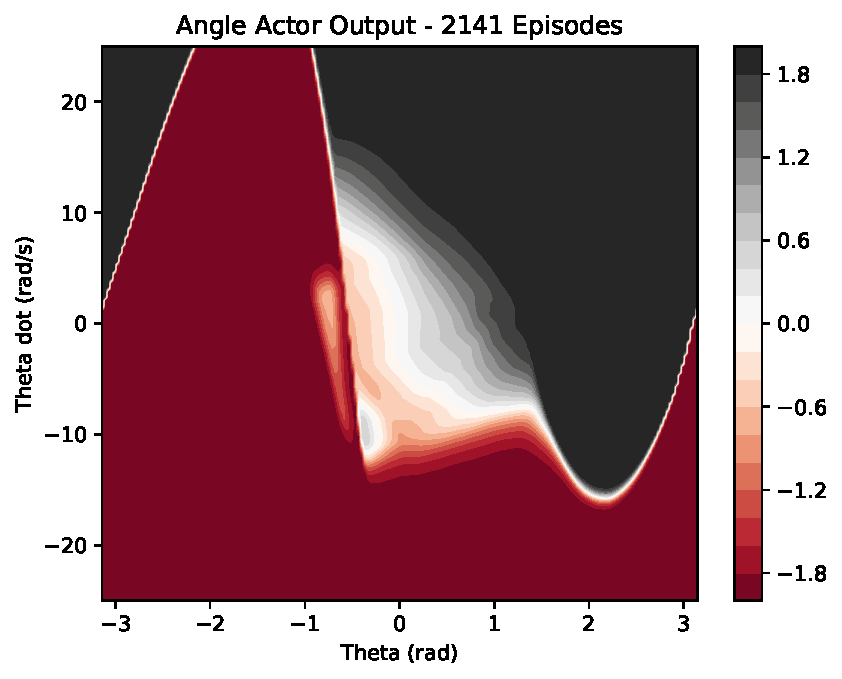
\includegraphics[width=65mm]{figures/train_figs/angle_actor/Actor0_2141.pdf} \\
	\end{tabular}
	\caption{caption}
\end{figure}

\begin{figure}[H]
	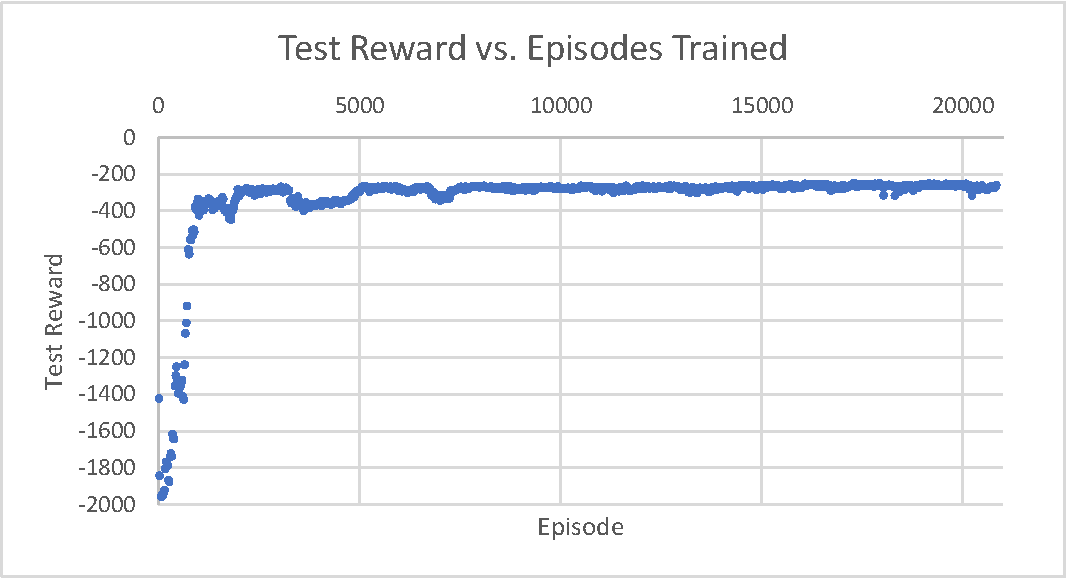
\includegraphics[width=6in, height=3.85in, keepaspectratio]{figures/train_figs/all_r.pdf}
	\caption{Training and Test Reward} \label{fig:all_r}
\end{figure}

\begin{figure}[H]
	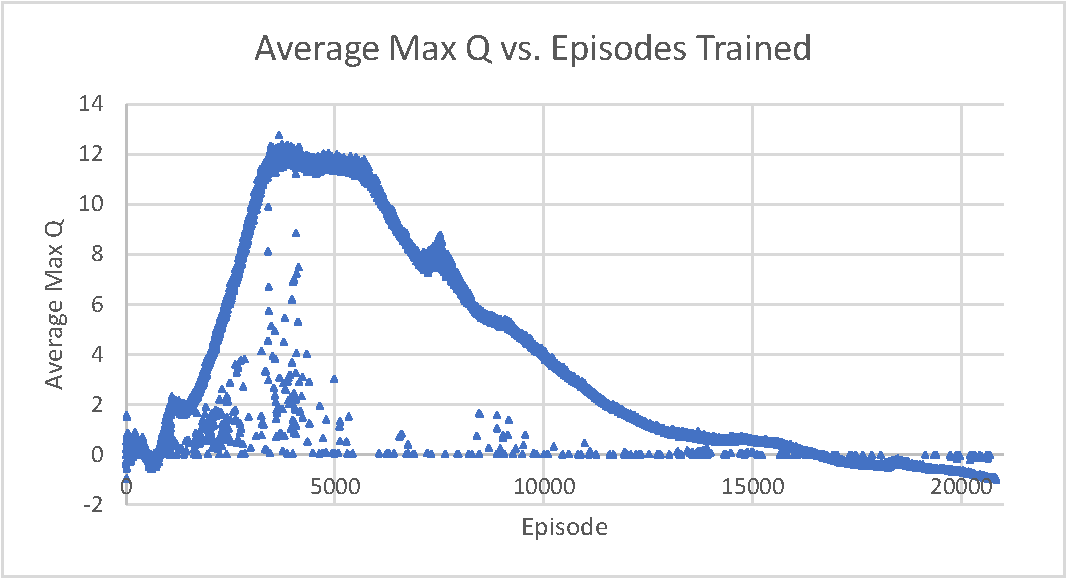
\includegraphics[width=6in, height=3.85in, keepaspectratio]{figures/train_figs/all_q.pdf}
	\caption{Average Max Q} \label{fig:all_q}
\end{figure}

